%%%%%%%%%%%%%%%%%%%%%%%%%%%%%%%%%%%%%%%%%%%%%%%%%%%%%%%%%%%%%%%
%% OXFORD THESIS TEMPLATE

% Use this template to produce a standard thesis that meets the Oxford University requirements for DPhil submission
%
% Originally by Keith A. Gillow (gillow@maths.ox.ac.uk), 1997
% Modified by Sam Evans (sam@samuelevansresearch.org), 2007
% Modified by John McManigle (john@oxfordechoes.com), 2015
% Modified by Ulrik Lyngs (ulrik.lyngs@cs.ox.ac.uk), 2018, for use with R Markdown
%
% Ulrik Lyngs, 25 Nov 2018: Following John McManigle, broad permissions are granted to use, modify, and distribute this software
% as specified in the MIT License included in this distribution's LICENSE file.
%
% John tried to comment this file extensively, so read through it to see how to use the various options.  Remember
% that in LaTeX, any line starting with a % is NOT executed.  Several places below, you have a choice of which line to use
% out of multiple options (eg draft vs final, for PDF vs for binding, etc.)  When you pick one, add a % to the beginning of
% the lines you don't want.


%%%%% CHOOSE PAGE LAYOUT
% The most common choices should be below.  You can also do other things, like replacing "a4paper" with "letterpaper", etc.

% This one will format for two-sided binding (ie left and right pages have mirror margins; blank pages inserted where needed):
%\documentclass[a4paper,twoside]{templates/ociamthesis}
% This one will format for one-sided binding (ie left margin > right margin; no extra blank pages):
%\documentclass[a4paper]{ociamthesis}
% This one will format for PDF output (ie equal margins, no extra blank pages):
%\documentclass[a4paper,nobind]{templates/ociamthesis}
%UL 2 Dec 2018: pass this in from YAML
\documentclass[a4paper, nobind]{templates/ociamthesis}


% UL 30 Nov 2018 pandoc puts lists in 'tightlist' command when no space between bullet points in Rmd file
\providecommand{\tightlist}{%
  \setlength{\itemsep}{0pt}\setlength{\parskip}{0pt}}
 
% UL 1 Dec 2018, fix to include code in shaded environments

%UL 2 Dec 2018 reduce whitespace around verbatim environments
\usepackage{etoolbox}
\makeatletter
\preto{\@verbatim}{\topsep=0pt \partopsep=0pt }
\makeatother

%UL 26 Mar 2019, enable strikethrough
\usepackage[normalem]{ulem}

%UL 15 Oct 2019, enable link highlighting to be turned off from YAML
\usepackage[colorlinks=false,pdfpagelabels,hidelinks=true]{hyperref}

%%%%% SELECT YOUR DRAFT OPTIONS
% Three options going on here; use in any combination.  But remember to turn the first two off before
% generating a PDF to send to the printer!

% This adds a "DRAFT" footer to every normal page.  (The first page of each chapter is not a "normal" page.)

% This highlights (in blue) corrections marked with (for words) \mccorrect{blah} or (for whole
% paragraphs) \begin{mccorrection} . . . \end{mccorrection}.  This can be useful for sending a PDF of
% your corrected thesis to your examiners for review.  Turn it off, and the blue disappears.
\correctionstrue

%%%%% BIBLIOGRAPHY SETUP
% Note that your bibliography will require some tweaking depending on your department, preferred format, etc.
% The options included below are just very basic "sciencey" and "humanitiesey" options to get started.
% If you've not used LaTeX before, I recommend reading a little about biblatex/biber and getting started with it.
% If you're already a LaTeX pro and are used to natbib or something, modify as necessary.
% Either way, you'll have to choose and configure an appropriate bibliography format...

% The science-type option: numerical in-text citation with references in order of appearance.
% \usepackage[style=numeric-comp, sorting=none, backend=biber, doi=false, isbn=false]{biblatex}
% \newcommand*{\bibtitle}{References}

% The humanities-type option: author-year in-text citation with an alphabetical works cited.
% \usepackage[style=authoryear, sorting=nyt, backend=biber, maxcitenames=2, useprefix, doi=false, isbn=false]{biblatex}
% \newcommand*{\bibtitle}{Works Cited}

%UL 3 Dec 2018: set this from YAML in index.Rmd
\usepackage[style=authoryear, sorting=nyt, backend=biber, maxcitenames=2, useprefix, doi=true, isbn=false, uniquename=false]{biblatex}
\newcommand*{\bibtitle}{Works Cited}

% This makes the bibliography left-aligned (not 'justified') and slightly smaller font.
\renewcommand*{\bibfont}{\raggedright\small}

% Change this to the name of your .bib file (usually exported from a citation manager like Zotero or EndNote).
\addbibresource{references.bib}


% Uncomment this if you want equation numbers per section (2.3.12), instead of per chapter (2.18):
%\numberwithin{equation}{subsection}


%%%%% THESIS / TITLE PAGE INFORMATION
% Everybody needs to complete the following:
\title{Determining the Influence of Different Variables on the Price of Ikea Products\\
-- a Regression Analysis}
\author{Philip Krück, Johannes Pein}
\college{}

% Master's candidates who require the alternate title page (with candidate number and word count)
% must also un-comment and complete the following three lines:
%\masterssubmissiontrue
%\candidateno{933516}
%\wordcount{28,815}

% Uncomment the following line if your degree also includes exams (eg most masters):
%\renewcommand{\submittedtext}{Submitted in partial completion of the}
% Your full degree name.  (But remember that DPhils aren't "in" anything.  They're just DPhils.)
\degree{B.Sc. Business Informatics (A Track)}
% Term and year of submission, or date if your board requires (eg most masters)
\degreedate{04.12.2020}


%%%%% YOUR OWN PERSONAL MACROS
% This is a good place to dump your own LaTeX macros as they come up.
\modulename{Digital Toolbox: Data Business}
\lecturer{Lecturer: Ulf Köther}
\groupnumber{Group Number: 7}
\matriculationnumbers{Matriculation Numbers: 3938 (P.Krück), **** (J.Pein)}


% To make text superscripts shortcuts
	\renewcommand{\th}{\textsuperscript{th}} % ex: I won 4\th place
	\newcommand{\nd}{\textsuperscript{nd}}
	\renewcommand{\st}{\textsuperscript{st}}
	\newcommand{\rd}{\textsuperscript{rd}}

%%%%% THE ACTUAL DOCUMENT STARTS HERE
\begin{document}

%%%%% CHOOSE YOUR LINE SPACING HERE
% This is the official option.  Use it for your submission copy and library copy:
\setlength{\textbaselineskip}{22pt plus2pt}
% This is closer spacing (about 1.5-spaced) that you might prefer for your personal copies:
%\setlength{\textbaselineskip}{18pt plus2pt minus1pt}

% You can set the spacing here for the roman-numbered pages (acknowledgements, table of contents, etc.)
\setlength{\frontmatterbaselineskip}{17pt plus1pt minus1pt}


% UL: You can set the general paragraph spacing here - I've set it to 2pt (was 0) so
% it's less claustrophobic
\setlength{\parskip}{2pt plus 1pt}


% Leave this line alone; it gets things started for the real document.
\setlength{\baselineskip}{\textbaselineskip}


%%%%% CHOOSE YOUR SECTION NUMBERING DEPTH HERE
% You have two choices.  First, how far down are sections numbered?  (Below that, they're named but
% don't get numbers.)  Second, what level of section appears in the table of contents?  These don't have
% to match: you can have numbered sections that don't show up in the ToC, or unnumbered sections that
% do.  Throughout, 0 = chapter; 1 = section; 2 = subsection; 3 = subsubsection, 4 = paragraph...

% The level that gets a number:
\setcounter{secnumdepth}{2}
% The level that shows up in the ToC:
\setcounter{tocdepth}{2}


% JEM: Pages are roman numbered from here, though page numbers are invisible until ToC.  This is in
% keeping with most typesetting conventions.
\begin{romanpages}

% Title page is created here
\maketitle

%%%%% MINI TABLES
% This lays the groundwork for per-chapter, mini tables of contents.  Comment the following line
% (and remove \minitoc from the chapter files) if you don't want this.  Un-comment either of the
% next two lines if you want a per-chapter list of figures or tables.
  \dominitoc % include a mini table of contents

% This aligns the bottom of the text of each page.  It generally makes things look better.
\flushbottom

% This is where the whole-document ToC appears:
\tableofcontents

%%%%% LIST OF ABBREVIATIONS
% This example includes a list of abbreviations.  Look at text/abbreviations.tex to see how that file is
% formatted.  The template can handle any kind of list though, so this might be a good place for a
% glossary, etc.
% First parameter can be changed eg to "Glossary" or something.
% Second parameter is the max length of bold terms.
\begin{mclistof}{List of Abbreviations}{3.2cm}

\item[R] Statistical Programming Language
\item[MSE] Mean Squared Error
\item[IQR] Interquartile Range

\end{mclistof} 


% The Roman pages, like the Roman Empire, must come to its inevitable close.
\end{romanpages}

%%%%% CHAPTERS
% Add or remove any chapters you'd like here, by file name (excluding '.tex'):
\flushbottom

% all your chapters and appendices will appear here
\hypertarget{intro}{%
\chapter{Introduction}\label{intro}}

\begin{figure}
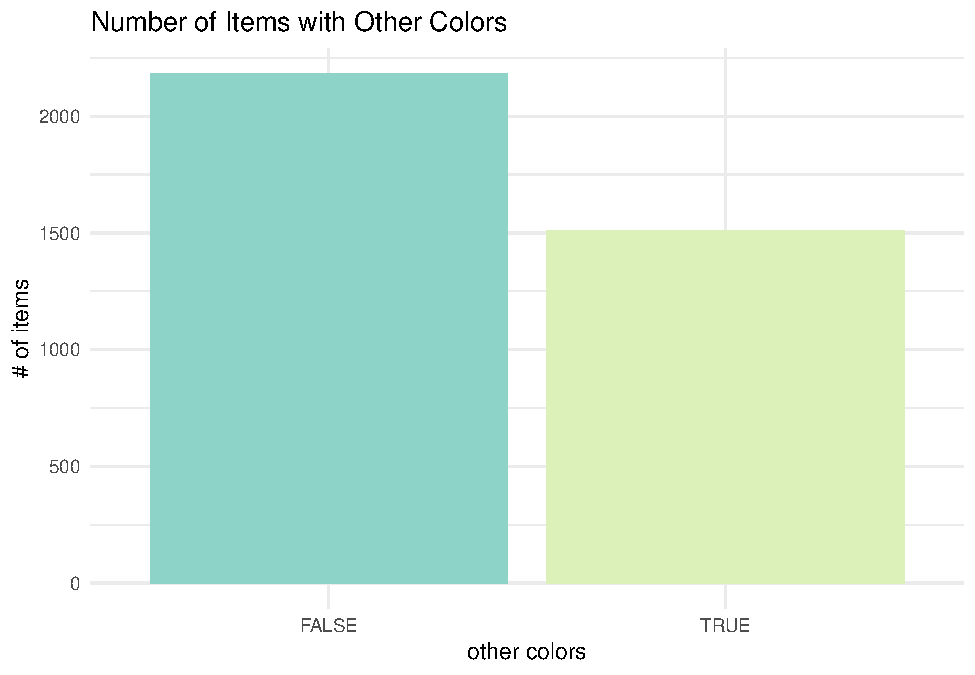
\includegraphics[width=1\linewidth]{_main_files/figure-latex/unnamed-chunk-3-1} \caption{Sample plot}\label{fig:unnamed-chunk-3}
\end{figure}

\hypertarget{theoretical-background-research-question}{%
\chapter{Theoretical Background \& Research Question}\label{theoretical-background-research-question}}

\hypertarget{theoretical_background}{%
\section{Theoretical Background}\label{theoretical_background}}

The data set was obtained by a kaggle.com user (Reem Abdulrahman) by the means of webscraping techniques from the Saudi Arabian Ikea website in the furniture category on the 20th of April 2020. Noteworthy features include the name, category, price in Saudi Riyals, the designer and dimensions (width, height and depth). The data set has 13 variables and 2962 observations.

\hypertarget{research_question}{%
\section{Research Question}\label{research_question}}

This paper explores the influence for different variables on the price in the given data set. The motivating forces for this research question are the possible implications for price determination of new items.

\hypertarget{methods}{%
\chapter{Methods}\label{methods}}

\hypertarget{datacleaning}{%
\section{Data Cleaning and Transformatoin}\label{datacleaning}}

To examine our data set properly, we first had to restructure and reformat it. This initial data cleaning step included type conversions, value mutation, addition of new calculated fields and the dropping of irrelevant columns.
Concretely, we converted name, category and designer to categorical variables. In the designer column, we converted blank strings and values prefixed by ``IKEA of Sweden'' to missing values (\texttt{NA}). Furthermore, we converted both the price and old price to double values and changed the currency from Saudi Arabian Riyals to Euros based on the exchange rate from the time the data set was obtained by the author @ref(\#theoretical\_background). To better facilitate the comparison of the different sizes of furniture items, we calcuted the size in cubic meters based on the depth, width and height values.
Finally, we selected only columns that could have a potential impact in our analysis (see Table \ref{tab:initial-ikea} and \ref{tab:tidy-ikea}).

TODO: Format these tables

\begin{table}

\caption{\label{tab:initial-ikea}Initial Data Set formatting.}
\centering
\begin{tabular}[t]{r|r|l|l|r|l|l|l|l|l|l|r|r|r}
\hline
X1 & item\_id & name & category & price & old\_price & sellable\_online & link & other\_colors & short\_description & designer & depth & height & width\\
\hline
0 & 90420332 & FREKVENS & Bar furniture & 2650 & No old price & TRUE & https://www.ikea.com/sa/en/p/frekvens-bar-table-in-outdoor-black-90420332/ & No & Bar table, in/outdoor,          51x51 cm & Nicholai Wiig Hansen & NA & 99 & 51\\
\hline
1 & 368814 & NORDVIKEN & Bar furniture & 9950 & No old price & FALSE & https://www.ikea.com/sa/en/p/nordviken-bar-table-black-00368814/ & No & Bar table,          140x80 cm & Francis Cayouette & NA & 105 & 80\\
\hline
2 & 9333523 & NORDVIKEN / NORDVIKEN & Bar furniture & 20950 & No old price & FALSE & https://www.ikea.com/sa/en/p/nordviken-nordviken-bar-table-and-4-bar-stools-black-black-s09333523/ & No & Bar table and 4 bar stools & Francis Cayouette & NA & NA & NA\\
\hline
3 & 80155205 & STIG & Bar furniture & 690 & No old price & TRUE & https://www.ikea.com/sa/en/p/stig-bar-stool-with-backrest-black-silver-colour-80155205/ & Yes & Bar stool with backrest,          74 cm & Henrik Preutz & 50 & 100 & 60\\
\hline
4 & 30180504 & NORBERG & Bar furniture & 2250 & No old price & TRUE & https://www.ikea.com/sa/en/p/norberg-wall-mounted-drop-leaf-table-white-30180504/ & No & Wall-mounted drop-leaf table,          74x60 cm & Marcus Arvonen & 60 & 43 & 74\\
\hline
5 & 10122647 & INGOLF & Bar furniture & 3450 & No old price & TRUE & https://www.ikea.com/sa/en/p/ingolf-bar-stool-with-backrest-white-10122647/ & No & Bar stool with backrest,          63 cm & Carina Bengs & 45 & 91 & 40\\
\hline
\end{tabular}
\end{table}

\begin{table}

\caption{\label{tab:tidy-ikea}Data Set after cleaning process.}
\centering
\begin{tabular}[t]{l|l|r|r|l|l|l|r}
\hline
name & category & price\_eur & old\_price\_eur & sellable\_online & other\_colors & designer & size\_m3\\
\hline
FREKVENS & Bar furniture & 65.02 & NA & TRUE & FALSE & Nicholai Wiig Hansen & NA\\
\hline
NORDVIKEN & Bar furniture & 244.14 & NA & FALSE & FALSE & Francis Cayouette & NA\\
\hline
NORDVIKEN / NORDVIKEN & Bar furniture & 514.05 & NA & FALSE & FALSE & Francis Cayouette & NA\\
\hline
STIG & Bar furniture & 16.93 & NA & TRUE & TRUE & Henrik Preutz & 0.30\\
\hline
NORBERG & Bar furniture & 55.21 & NA & TRUE & FALSE & Marcus Arvonen & 0.19\\
\hline
INGOLF & Bar furniture & 84.65 & NA & TRUE & FALSE & Carina Bengs & 0.16\\
\hline
\end{tabular}
\end{table}

\hypertarget{tbd}{%
\section{8 Step EDA (nice heading)}\label{tbd}}

Here we describe our EDA after the ZUUR paper method \autocite[pp.~33-35]{von_goethe_wilhelm_1829}.
Lorem ipsum dolor sit amet, consetetur sadipscing elitr, sed diam nonumy eirmod tempor invidunt ut labore et dolore magna aliquyam erat, sed diam voluptua. At vero eos et accusam et justo duo dolores et ea rebum. Stet clita kasd gubergren, no sea takimata sanctus est Lorem ipsum dolor sit amet. Lorem ipsum dolor sit amet, consetetur sadipscing elitr, sed diam nonumy eirmod tempor invidunt ut labore et dolore magna aliquyam erat, sed diam voluptua. At vero eos et accusam et justo duo dolores et ea rebum. Stet clita kasd gubergren, no sea takimata sanctus est Lorem ipsum dolor sit amet.Lorem ipsum dolor sit amet, consetetur sadipscing elitr, sed diam nonumy eirmod tempor invidunt ut labore et dolore magna aliquyam erat, sed diam voluptua. At vero eos et accusam et justo duo dolores et ea rebum. Stet clita kasd gubergren, no sea takimata sanctus est Lorem ipsum dolor sit amet. Lorem ipsum dolor sit amet, consetetur sadipscing elitr, sed diam nonumy eirmod tempor invidunt ut labore et dolore magna aliquyam erat, sed diam voluptua. At vero eos et accusam et justo duo dolores et ea rebum. Stet clita kasd gubergren, no sea takimata sanctus est Lorem ipsum dolor sit amet.

\hypertarget{step-1}{%
\subsection{Step 1}\label{step-1}}

Lorem ipsum dolor sit amet, consetetur sadipscing elitr, sed diam nonumy eirmod tempor invidunt ut labore et dolore magna aliquyam erat, sed diam voluptua. At vero eos et accusam et justo duo dolores et ea rebum. Stet clita kasd gubergren, no sea takimata sanctus est Lorem ipsum dolor sit amet. Lorem ipsum dolor sit amet, consetetur sadipscing elitr, sed diam nonumy eirmod tempor invidunt ut labore et dolore magna aliquyam erat, sed diam voluptua. At vero eos et accusam et justo duo dolores et ea rebum. Stet clita kasd gubergren, no sea takimata sanctus est Lorem ipsum dolor sit amet.

\hypertarget{step-2}{%
\subsection{Step 2}\label{step-2}}

\hypertarget{step-3}{%
\subsection{Step 3}\label{step-3}}

\hypertarget{step-4}{%
\subsection{Step 4}\label{step-4}}

\hypertarget{step-5}{%
\subsection{Step 5}\label{step-5}}

\hypertarget{step-6}{%
\subsection{Step 6}\label{step-6}}

\hypertarget{step-7}{%
\subsection{Step 7}\label{step-7}}

\hypertarget{step-8}{%
\subsection{Step 8}\label{step-8}}

\hypertarget{tbd2}{%
\section{Random Forest Regression Model}\label{tbd2}}

Lorem ipsum dolor sit amet, consetetur sadipscing elitr, sed diam nonumy eirmod tempor invidunt ut labore et dolore magna aliquyam erat, sed diam voluptua. At vero eos et accusam et justo duo dolores et ea rebum. Stet clita kasd gubergren, no sea takimata sanctus est Lorem ipsum dolor sit amet. Lorem ipsum dolor sit amet, consetetur sadipscing elitr, sed diam nonumy eirmod tempor invidunt ut labore et dolore magna aliquyam erat, sed diam voluptua. At vero eos et accusam et justo duo dolores et ea rebum. Stet clita kasd gubergren, no sea takimata sanctus est Lorem ipsum dolor sit amet.

\hypertarget{results}{%
\chapter{Results}\label{results}}

Lorem ipsum dolor sit amet, consetetur sadipscing elitr, sed diam nonumy eirmod tempor invidunt ut labore et dolore magna aliquyam erat, sed diam voluptua. At vero eos et accusam et justo duo dolores et ea rebum. Stet clita kasd gubergren, no sea takimata sanctus est Lorem ipsum dolor sit amet. Lorem ipsum dolor sit amet, consetetur sadipscing elitr, sed diam nonumy eirmod tempor invidunt ut labore et dolore magna aliquyam erat, sed diam voluptua. At vero eos et accusam et justo duo dolores et ea rebum. Stet clita kasd gubergren, no sea takimata sanctus est Lorem ipsum dolor sit amet.

\hypertarget{discussion}{%
\chapter{Discussion}\label{discussion}}

Lorem ipsum dolor sit amet, consetetur sadipscing elitr, sed diam nonumy eirmod tempor invidunt ut labore et dolore magna aliquyam erat, sed diam voluptua. At vero eos et accusam et justo duo dolores et ea rebum. Stet clita kasd gubergren, no sea takimata sanctus est Lorem ipsum dolor sit amet. Lorem ipsum dolor sit amet, consetetur sadipscing elitr, sed diam nonumy eirmod tempor invidunt ut labore et dolore magna aliquyam erat, sed diam voluptua. At vero eos et accusam et justo duo dolores et ea rebum. Stet clita kasd gubergren, no sea takimata sanctus est Lorem ipsum dolor sit amet.

\hypertarget{individual-statements}{%
\chapter{Individual Statements}\label{individual-statements}}

\hypertarget{philip-kruxfcck}{%
\section{Philip Krück}\label{philip-kruxfcck}}

\hypertarget{johannes-pein}{%
\section{Johannes Pein}\label{johannes-pein}}

\startappendices

\hypertarget{plots}{%
\chapter{Plots}\label{plots}}

\hypertarget{plot-xyz}{%
\section{Plot xyz}\label{plot-xyz}}

\hypertarget{plot-abc}{%
\section{Plot abc}\label{plot-abc}}

\hypertarget{another-appendix}{%
\chapter{Another Appendix}\label{another-appendix}}


%%%%% REFERENCES

% JEM: Quote for the top of references (just like a chapter quote if you're using them).  Comment to skip.
% \begin{savequote}[8cm]
% The first kind of intellectual and artistic personality belongs to the hedgehogs, the second to the foxes \dots
%   \qauthor{--- Sir Isaiah Berlin \cite{berlin_hedgehog_2013}}
% \end{savequote}

\setlength{\baselineskip}{0pt} % JEM: Single-space References

{\renewcommand*\MakeUppercase[1]{#1}%
\printbibliography[heading=bibintoc,title={\bibtitle}]}

\end{document}
